\section{Méthodes d'identification de mèmes dans un large volume de donneés}

Choisir un ensemble de mèmes cohérents est une des étapes difficiles de notre recherche. En effet, dans le vaste corpus de données utilisées et plus généralement dans la multitude des échanges quotidiens sur les réseaux sociaux, trouver une prise pour l{\textquoteright}étude n{\textquoteright}est pas une t\^ache évidente. Cette section présente les résultats obtenus lors de différentes approches pour constituer des corpus de données représentatifs de mèmes dans un large volume de données.

\subsection[Constitution et collection d{\textquoteright}un corpus de messages]{Constitution et collection d{\textquoteright}un corpus de messages}
\label{sec:weiboscope}
La première question qui se pose à nous est le choix du corpus de données à utiliser.

Afin de poursuivre notre étude, nous allons donc procéder à l{\textquoteright}analyse de données issues de services de réseaux sociaux en ligne. La plupart des services de réseaux sociaux en ligne offrent un large accès car il s{\textquoteright}agit souvent de la fondation de leurs modèles d{\textquoteright}affaires basés sur la valorisation et la revente de ces données pour le marketing ciblé \citep{Ko2010}. Pour entrer en contact avec la base de données, les SNS mettent à disposition une API (\textit{Application Programming Interface}) qui permet à un programme ou une autre application web de se connecter au service pour demander et obtenir des données. L{\textquoteright}API est donc la première source d{\textquoteright}obtention de données depuis les SNS. Néanmoins, les données des réseaux sociaux sont soumises à d{\textquoteright}importants enjeux et contraintes tant commerciales, éthiques que politiques dans le cas de la Chine notamment. Les conditions d{\textquoteright}utilisations techniques et légales (\textit{Terms of Uses) }de ces données sont également soumises à des changements fréquents, étroitement liés à l{\textquoteright}évolution commerciale et technologique de compagnies souvent très jeunes. Nous avons établi une liste des limitations et écueils pouvant \^etre rencontrés lors de l{\textquoteright}extraction et de l{\textquoteright}analyse de données des SNS :

\begin{description}
    
    \item[Compatibilité] Une solution technologique devient facilement caduque lors de l{\textquoteright}évolution d{\textquoteright}une API (ex. Twitter APi v1.0 n{\textquoteright}existe plus, ainsi le code doit \^etre réécrit pour la version 1.1).  
    
    \item [Disponibilité] : Chaque API répond à des formats et critères précis et possède ses propres limitations. Pour accéder à l{\textquoteright}API du moteur de recherche de Sina Weibo, il faut s{\textquoteright}identifier auprès de la compagnie gr\^ace à une carte d{\textquoteright}identité et des paiements par requ\^ete sont exigés.

    \item[Limitations d{\textquoteright}usage] : Afin de limiter le trafic et conserver le contr\^ole sur les données distribuées, les SNS mettent en place des limitations d{\textquoteright}accès à leurs serveurs, notamment : limitation du nombre de requ\^etes par heure, limitation du nombre de requ\^etes par machine (basée sur l{\textquoteright}adresse IP), limitation du nombre d{\textquoteright}utilisateurs connectés. Ainsi, Twitter limite à 150 requ\^etes API par heure pour un compte non identifié, pouvant augmenter jusqu{\textquoteright}à 500 après authentification. Les données datant de plus de 7 jours sont payantes, reflétant la valeur d{\textquoteright}un accès en {\textquotedblleft}temps-réel{\textquotedblright} aux données.
    
    \item[Légalité ] Les données sont soumises aux conditions de propriété décrites légalement par la firme qui les publient \citep{Clifton2006}. Ces conditions sont susceptibles de changer. Ainsi, Twitter a exigé en 2012 le retrait a posteriori de nombreux jeux de données publiés par des chercheurs depuis plusieurs années parfois \citep{McCreadie2012}. Actuellement, Twitter précise notamment dans ses \textit{Terms of Use: {\textquotedblleft}You may not resyndicate or share Twitter content, including datasets of Tweet text and follow relationships{\textquotedblright} }\footnote{ Terms of use de Twitter, \url{https://dev.twitter.com/terms/api-terms}, consulté le 12 Mars 2013 à 17h08}.
    
    \item[Ethique] Vous pouvez extraire depuis une API des profils d{\textquoteright}utilisateurs contenant les informations qu{\textquoteright}ils ont auparavant publié en ligne (Felt \& Evans,  2008). En exposant les données personnelles des utilisateurs, le chercheur est responsable de l{\textquoteright}usage qu{\textquoteright}il fait des données \citep{Rieder2005}  
\end{description}

Afin d{\textquoteright}obtenir des données et de contourner les limitations de l{\textquoteright}API, la pratique dite du \textit{{\textquotedblleft}scraping{\textquotedblright} }permet d{\textquoteright}obtenir des données à l{\textquoteright}aide d{\textquoteright}un robot qui lit et sauvegarde des parties ou l{\textquoteright}intégralité de pages web. Les moteurs de recherche utilisent notamment cette technique pour l{\textquoteright}indexation des pages. Ce type de pratiques est également soumis à des limitations par les services web (blocage de l{\textquoteright}IP source) et se situe à la limite de la légalité,voire est explicitement interdite dans le cas de certains SNS \citep{Petschulat2010}.

Un programme appelé \textit{spider }ou \textit{crawler} est chargé d{\textquoteright}effectuer des requ\^etes régulières à l{\textquoteright}API afin d{\textquoteright}obtenir et collecter les informations obtenues dans une base de données. Plusieurs approches existent dans les techniques échantillonnage de réseau social. La première, fondée sur des mots-clés extraits les posts contenant des mots ou des hashtags particuliers. La seconde utilise l{\textquoteright}échantillonnage de graphe, collectant au fil des liens les conversations ou profils des utilisateurs. Classique des études statistiques, cet échantillonage dit \textit{boule de neige {\textquotedblleft}élargit l{\textquoteright}échantillon en partant d{\textquoteright}un node original pour s{\textquoteright}éloigner vers ses voisins{\textquotedblright}} \citep{Rothenberg1995}. Ici, deux grandes catégories s{\textquoteright}opposent : les techniques traversales o\`u les nodes sont classifiés après avoir été visités et les {\textquotedblleft}walk{\textquotedblright} aléatoires o\`u l{\textquoteright}extension du graphe visité se fait de manière aléatoire \citep{Gjoka2011}.

Au cours du travail préparatoire de cette recherche, nous avons tout d{\textquoteright}abord expérimenté plusieurs algorithmes et outils de collection de données afin d{\textquoteright}en comparer les résultats. Une première approche d{\textquoteright}extraction par utilisateurs a été infructueuse car la sélection du groupe source (\textit{seeds}) ne permettait pas d{\textquoteright}obtenir des résultats cohérents\footnote{ Code disponible : \url{https://github.com/sharismlab/Pyweibo}, consulté le 14 Mars à 5h32}. Par la suite, une autre approche de collecte de données via le développement d{\textquoteright}un plug-in pour le navigateur Google Chrome\footnote{ Code disponible : \url{https://github.com/sharismlab/battlefield}, consulté le 14 Mars à 5h12\par } nous a permis de tester et d{\textquoteright}apercevoir les limites de la collection de données par mots-clés. Cette étape nous a également montré l{\textquoteright}intér\^et que peut présenter une approche collaborative de la collection de données ou de seeds par un système de {\textquotedblleft}curation{\textquotedblright} collaboratifs afin d{\textquoteright}obtenir des éléments précis de contenus et de réduire la masse de données inutiles qui pollue souvent les jeux de données \citep{Ding2013}. Après de multiples tests et comparaisons d{\textquoteright}outils et de librairies, plusieurs difficultés majeures limitaient l{\textquoteright}obtention d{\textquoteright}une quantité de données suffisantes, notamment la nécessité de ressources assez importantes (en terme de développement et de disponibilité des machines), un temps d{\textquoteright}acquisition parfois très long et l{\textquoteright}exigence d{\textquoteright}une veille constante sur les SNS pour identifier un mème au bon moment (les tweets de Sina Weibo devenant indisponibles via l{\textquoteright}API au-delà de 7 jours). La première limite se situe bien s\^ur dans la capacité d{\textquoteright}une personne seule à mener à bien cette large t\^ache. Nous avons donc choisi de considérer les jeux de données collectés sur Sina Weibo disponibles sur l{\textquoteright}Internet. Une fois écartés les nombreux jeux tronqués, modifiés ou incomplets, nous avons pu obtenir plusieurs jeux de données provenant de recherches préalables dans le domaine particulier de l{\textquoteright}échantillonnage \citep{Ding2013} ou ayant servi de bases à des études précédentes \citep{Gao2012}. Finalement, nous avons identifié le jeu de données constitué lors du projet \textit{Weiboscope }de l{\textquoteright}Université de Hong Kong comme répondant à nos besoins en termes de dimensions (temps, nombre d{\textquoteright}utilisateurs observés), taille (nombre de tweets) et contenus (géo-localisation, présence des tweets censurés).


Notre travail d{\textquoteright}analyse s{\textquoteright}appuie donc sur ce jeu de données collecté sur le service de microblog Sina Weibo par le \textit{Journalism and Media Studies Centre} (JMSC) de l{\textquoteright}Université de Hong Kong lors de son projet \textit{Weiboscope}. Téléchargeable ouvertement, la publication de ce jeu de données a pour objectif de \textit{{\textquotedblleft}enables academic use of the data for better understanding of the social }\textit{media in China and making the Chinese media system more transparent.{\textquotedblright}}\footnote{ Le jeu de données Weiboscope est disponible à l{\textquoteright}adresse : \url{http://147.8.142.179/datazip/}, consulté le 14 Mars à 17h21 }\textit{ }Il s{\textquoteright}agit d{\textquoteright}un échantillonnage aléatoire de messages \textit{(random sampling)} effectué quotidiennement durant toute l{\textquoteright}année 2012 sur un panel d{\textquoteright}environ 350 000 utilisateurs ayant au moins 1000 followers \citep{Fu2013}. La totalité du jeu de données comprend 226,841,122 messages répartis sur 52 semaines, dont des messages ayant été supprimés par les utilisateurs eux-m\^emes ou par les administrateurs de Sina Weibo eux-m\^emes - parfois sur ordre du gouvernement chinois (\textit{ibid}, 2013).

\begin{table}[ht]
    \centering
    \small
    \begin{tabulary}{\textwidth}{c|C} 
        \toprule
        \textbf{Désignation}
        & \textbf{Description} \\
        \hline \\[-1.5ex]

        mid  &
        Unique pseudo message ID\\[2ex]
        retweeted\_status\_mid  &
        Pseudo message ID of the original message (Only available if the row of
        interest is a retweet)\\[2ex]
        Uid &
        Pseudo user ID\\[2ex]
        retweeted\_uid &
        Pseudo user ID of the original poster (Only available if the row of
        interest is a retweet)\\[2ex]
        Source &
        The application name of the client program\\[2ex]
        Image &
        With image? (1= Yes, 0=No)\\[2ex]
        text  &
        body of the message. Any address handle (@xxxx:) is replaced by either
        the pseudo user ID or ukn (uknown)\\[2ex]
        geo &
        GIS information. Please refer to the Sina Weibo API documentation:
        \url{http://goo.gl/Um8SS}\\[2ex]
        created\_at &
        Original posting time\\[2ex]
        deleted\_last\_seen &
        The last seen time before this message was missing from the user
        timeline\\[2ex]
        permission\_denied  &
        {\textquotesingle}permission denied{\textquotesingle} status is marked
        when the message was found missing in the timeline and the API return
        message was {\textquotesingle}permission denied{\textquotesingle} - See
        details in (Fu, Chan, Chau 2013)\\[2ex]
    \end{tabulary}
    \caption[Modèle de messages pour le jeu de données Weiboscope]{Modèle de messages pour le jeu de données Weiboscope}
\end{table}

Ce jeu de données a été mis à disposition sous une forme anonymisée o\`u les identifiants des messages et des utilisateurs ont été remplacés par des pseudo-identifiants. La collection des données a été effectuée sur une série d{\textquoteright}utilisateurs (génération aléatoire d{\textquoteright}identifiants dont l{\textquoteright}existence est ensuite validée) pour donner \textit{{\textquotedblleft}une image représentative des usages et utilisateurs de Sina Weibo (...) dont les études auparavant limitée à des analyses non-aléatoire (...) se cantonnaient aux utilisateurs les plus populaires{\textquotedblright} }\citep{Fu2013}. Ainsi, plut\^ot que de considérer uniquement les {\textquotedblleft}stars{\textquotedblright} de Sina Weibo, cet échantillon s{\textquoteright}attache à refléter également les pratiques des utilisateurs {\textquotedblleft}lambda{\textquotedblright}. Ce jeu de données a déjà été partiellement étudié dans le but de comprendre la démographie des utilisateurs de Sina Weibo, leurs activités et les comportements pouvant permettre de prédire les réactions notamment de censure. La démographie des utilisateurs se composent de 55\% d{\textquoteright}hommes habitant principalement dans les grandes villes de Chine (Pékin, Canton, Shanghai). Une des découvertes importantes est le très faible taux de création originale de messages malgré une activité importante des utilisateurs, indiquant que l{\textquoteright}essentiel de l{\textquoteright}activité sur Sina Weibo se constitue de re-posts et de commentaires \citep{Fu2013}. Le jeu de données est accompagné des informations succintes de profil des utilisateurs dont le lieu, rempli par eux, sans néanmoins fournir leurs noms d{\textquoteright}utilisateur véritables. Notre travail de recherche s{\textquoteright}articule autour d{\textquoteright}une nouvelle lecture de ce jeu de données unique.

\subsection[Détection algorithmique de mèmes]{Détection algorithmique de mèmes dans un large corpus de données}
\label{sec:protomemes}

Une fois l{\textquoteright}acquisition des données effectuées, il s{\textquoteright}agit désormais de savoir les analyser correctement pour y déceler les mèmes que nous souhaitons considérer. Les travaux dans le domaine de la détection et l{\textquoteright}identification de mèmes dans les données de réseaux sociaux restent encore peu nombreux. Une des études pionnières est l{\textquoteright}outil \textit{MemeTracker }(devenu \textit{NIFTY}) con\c{c}u en 2009 par le \textit{SNA Project }de l{\textquoteright}Université de Stanford \citep{Leskovec2009}. Cet outil permet une étude sous forme de graphes de la diffusion de phrases dans un vaste corpus de texte mais n{\textquoteright}est pas adapté à la langue chinoise. La discussion sur la modélisation mathématiques des mèmes \citep{Ahmad2006, Nye2011} émane souvent de recherches en informatique cherchant à prendre en considération différents facteurs de diffusion lors de l{\textquoteright}analyse machine de données \citep{Zubiaga2011, Wang2011}, considérant le mème comme un vecteur de modification du réseau lui-m\^eme \citep{Ienco2010}. Plus marginal, des études s{\textquoteright}intéressent aux dynamiques géographiques des mèmes \citep{Kamath2013}. Néanmoins, aucune de ces différentes approches ne permet d{\textquoteright}apporter une réponse technologique ou algorithmique satisfaisante pour l{\textquoteright}identification de mèmes Internet dans un ensemble de données issu des réseaux sociaux. Afin de déceler les mèmes dans un vaste ensemble textuel, nous devons y déceler des motifs de diffusion particuliers. La dénomination \textit{machine learning }regroupe un ensemble d{\textquoteright}algorithmes qui permettent d{\textquoteright}explorer des jeux de données pour en extraire des représentations et y identifier des propriétés (\textit{features}) particulières. Basé sur les sciences statistiques, ces algorithmes font usage de mesures de similarité pour classifier les éléments d{\textquoteright}un corpus. Les catégories utilisées pour la classification peuvent \^etre définies au préalable par l{\textquoteright}utilisateur - c{\textquoteright}est le \textit{{\textquotedblleft}supervised learning{\textquotedblright} }ou inférées du jeu de données lui-m\^eme dans le cas du \textit{{\textquotedblleft}unsupervised learning{\textquotedblright}} pour la détection de \textit{clusters }\citep{Breiman2001}\textit{. }La multitude d{\textquoteright}algorithmes de \textit{machine learning }disponibles pour la détection de clusters au sein d{\textquoteright}un corpus textuel ou d{\textquoteright}un réseau social \citep{Nettleton2013, Robins2013} rend l{\textquoteright}identification d{\textquoteright}une solution difficile. De plus, les algorithmes utilisés traditionnellement pour l{\textquoteright}analyse de documents textuels (\textit{topic modeling, LSA}) se heurtent au caractère très disparate des corpus issus des réseaux sociaux (\textit{text sparsity issue) }faisant diminuer drastiquement leur efficacité \citep{Hong2010}.


Ferrara \& al. \citep{Ferrara2013} propose dans un papier intitulé {\textquotedblleft}\textit{Meme clustering in social media}{\textquotedblright} un algorithme utilisant la classification automatique non-supervisée pour détecter des mèmes dans un corpus de données de réseaux sociaux. Ce travail récent propose de tenir compte non seulement des textes et hashtags, mais aussi des liens et des modèles de diffusion pour identifier des groupes de messages intéressants et procéder au \textit{clustering }des mèmes. L{\textquoteright}algorithme s{\textquoteright}articule autour du concept de {\textquotedblleft}protomèmes{\textquotedblright}, représentant les éléments fondamentaux d{\textquoteright}un mème en cours de création \citep{Gabora1995}. Dans le contexte des médias sociaux, le protomème est défini par les entités (liens, hashtags...), mots-clés et séquences de conversation qui constitue le mème en devenir. En identifiant puis comparant les différents protomèmes présents dans chaque tweet, il est possible d{\textquoteright}y détecter des similarités et de deviner les mèmes en formation.  

\begin{figure} 
    \centering
    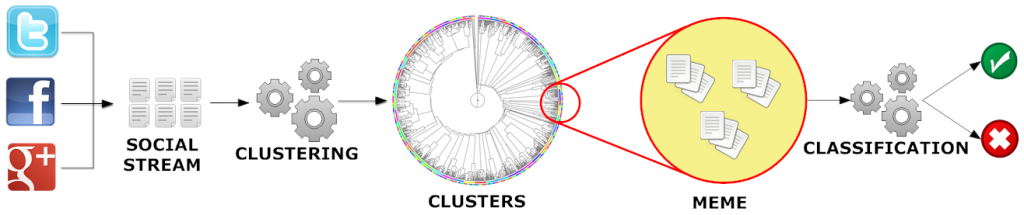
\includegraphics[width=5.8894in,height=1.2114in]{figures/chap3/chapitre3-img6.png}
    \caption{Algorithme de reconnaissance de mème (clustering) \citep{Ferrara2013}}
\end{figure}

Cet algorithme suppose donc d{\textquoteright}extraire dans un premier temps les éléments remarquables du corpus de tweets afin d{\textquoteright}établir des représentations de ces protomèmes contenant les éléments à comparer : \textit{phrases} (texte brut), \textit{mentions }(@, RT), \textit{hashtags }et \textit{urls}. Pour constituer ces jeux de protomèmes, nous utilisons le pattern \textit{map-reduce} qui permet de chercher et lister des éléments dans un vaste jeu de données \textit{(map)} avant de les regrouper dans une liste \textit{(reduce)}. Une fois ces protomèmes constitués nous procédons à leurs comparaisons selon plusieurs critères :

\begin{itemize}
\item \textit{Similarité de texte }: comparant le contenu texuel de chaque protomème 
\item \textit{Similarité d{\textquoteright}utilisateurs} : comparant les utilisateurs contenus dans chaque protomème
\item \textit{Similarités de tweet }: recherchant les tweets identiques dans différents protomèmes
\item \textit{Similarité de diffusion : }considérant les références aux utilisateurs contenus dans chaque protomème
\end{itemize}

Ici nous utilisons la \textit{sémantique vectorielle} (Support Vector Machine) afin de comparer les éléments des protomèmes gr\^ace à une représentation algébrique sous formes de vecteurs. Pratique ancienne de l{\textquoteright}algèbre linéaire appliquée à la science informatique \citep{Salton1975}, il s{\textquoteright}agit de permettre la conversion d{\textquoteright}objets textuels (mots, identifiants, images...) sous une forme aisément comparable. Pour convertir le texte sous forme vectorielle, l{\textquoteright}algorithme classique Tf-idf (\textit{Term Frequency - Inverse Document Frequency}) est utilisé \citep{Soucy2005}. Les autres mesures de similarité sont la \textit{mesure cosine (}ou \textit{similarité cosinus) }des protomèmes convertis sous forme de vecteurs binaires. Une fois ces différentes valeurs de similarité calculées, nous utilisons les scalaires définis dans le papier de référence pour assigner des poids à chacun des vecteurs et les combiner en une seule valeur \citep{Ferrara2013}. Cette matrice de valeurs de similarité nous permet alors de définir les protomèmes les plus similaires et d{\textquoteright}identifier ainsi des \textit{clusters }dans les données correspondant aux mèmes.


Si cette approche offre des résultats probants sur de petits volumes (quelques centaines de tweets), la très grande demande en puissance de calcul et ressources mémoires nécessaires rendent le traitement d{\textquoteright}un jeu données plus vaste irréalisable. Les opérations de comparaison et le calcul de similarités sur de vastes volumes de données font cro\^itre très rapidement la complexité des algorithmes et ainsi la quantité de calculs à effectuer. Le calcul du co\^ut d{\textquoteright}un algorithme se fait au travers des notions dites de domination, avec notamment le {\textquotedblleft}grand O{\textquotedblright} exprimé \textit{O(f(n)) }qui fait correspondre à la complexité d{\textquoteright}un algorithme une fonction \textit{f} de la quantité d{\textquoteright}information manipulée \textit{n. }Ainsi pour un algorithme courant de complexité \textit{O(n}\textit{\textsuperscript{2}}\textit{), }les ressources de calcul \textit{(computation)} et de mémoire (RAM ou stockage) nécessaires augmentent de manière exponentielle à chaque élément ajouté au corpus \textit{n}. L{\textquoteright}algorithme de {\textquotedblleft}meme clustering{\textquotedblright} décrit par Ferrara atteint donc un co\^ut exorbitant devant un large volume de données comme celui du jeu Weibosope. La limite physique de calcul est rapidement atteinte rendant impossible le franchissement du pallier expérimental et la vérification des hypothèses de travail à une échelle suffisante.

\subsection[Les hashtags ne sont pas des mèmes]{Les hashtags : artefacts de campagnes de communication planifiées}
\label{sec:hashtags}

Les travaux en sciences humaines sur les mèmes \citep{Bauckhage2011, Coscia2013, Knobel2007} et les sites spécialisés \citep{Buchel2012, Bernstein2011} présentent bien souvent un mème sous la forme d{\textquoteright}un titre (mot ou groupe de mots) accompagné d{\textquoteright}une collection d{\textquoteright}images ou/et de vidéos, ainsi qu{\textquoteright}un texte explicatif (mise en contexte) et des indications sur les dates de parution et son évolution dans le temps. Ici, un ou des auteurs se saisissent des matériaux bruts du web et les rassemblent pour reconstituer une vision particulière du mème, aussi représentative que possible. Cette approche nécessite peu de déploiement technologique (un copier/coller suffit souvent), mais exige néanmoins une forte connaissance et un suivi régulier du terrain Internet pour y dénicher ces représentations du mèmes. Cette démarche que nous nommerons \textit{ethnographique }s{\textquoteright}apparente à de la curation de contenu \citep{Buckingham2006}. Les \textit{hashtags }(en fran\c{c}ais {\textquotedblleft}mots-dièses{\textquotedblright}) sont utilisés dans l{\textquoteright}écriture sur les réseaux sociaux et se présentent dans Sina Weibo sous la forme d{\textquoteright}un mot entouré de deux dièses - ex. \textit{\#mot-clé\#}. Marqueur particulier, le hashtag permet à un interlocuteur de procéder à une dénotation ou connotation du message original \citep{Romero2011} ou d{\textquoteright}affirmer son caractère évènementiel (lors d{\textquoteright}un évènement sportif, d{\textquoteright}une conférence, etc). Facile à identifier dans la masse des données en ligne, il permet de désigner un ensemble de contenus sous un m\^eme signe. Ainsi, il est un vecteur important permettant de collecter simplement une large masse d{\textquoteright}informations autour d{\textquoteright}un mème. La constitution d{\textquoteright}un corpus autour d{\textquoteright}un {\textquotedblleft}hashtag{\textquotedblright} présente néanmoins plusieurs limites. Premièrement, le mème est par définition un objet en mutation. Ainsi, il est souvent difficile de l{\textquoteright}identifier une bonne fois pour toute par un ou plusieurs de mot-clés. De plus, le mème existe bien souvent sous la forme d{\textquoteright}images ou de vidéos qui ne sont pas nécessairement légendées ou référencées et donc peu accessible à une recherche {\textquotedblleft}plein texte{\textquotedblright}. Ainsi, une approche pour la recherche de mèmes ne peut \^etre entièrement textuelle et doit s{\textquoteright}intéresser aux autres forme de contenus web (notamment les liens et les hashtags). De plus, l{\textquoteright}ajout de hashtags dans les messages est un acte volontaire non systématique. Ainsi, si l{\textquoteright}identification de certains mèmes peut se faire gr\^ace à la recherche de hashtags, l{\textquoteright}ensemble des messages contenant des hashtags ne recouvrent pas systématiquement un mème. Comme nous le verrons, les hashtags sont bien souvent de simples artefacts de campagne marketing en ligne.

Afin de procéder à l{\textquoteright}analyse des mèmes, nous avons donc indexé l{\textquoteright}ensemble des contenus du corpus Weiboscope contenant des hashtags sur toute l{\textquoteright}année 2012 (30 millions sur un total de 200 millions tweets environs). Nous avons donc dans un premier temps extrait l{\textquoteright}ensemble des messages contenant un ou des hashtags de l{\textquoteright}ensemble des données avant de les classifier pour obtenir des jeux de données cohérents par hashtags. Une première contrainte ici est propre au traitement informatique de la langue chinoise qui constitue le langage majoritaire de notre corpus. L{\textquoteright}absence d{\textquoteright}espace entre les différents caractères de la phrase en chinois oblige à prendre en compte la sémantique de la phrase pour procéder à sa segmentation. Cette question usuelle pour les usagers du NLP (\textit{Natural Language Processing}) en chinois est un sujet de recherche encore très discuté \citep{Qiu2013}. L{\textquoteright}identification de la meilleure option parmi la multitude des librairies et logiciels disponibles pour la segmentation puis le NLP en chinois a été un aspect préliminaire importants de notre travail d{\textquoteright}analyse de données. Nous avons ainsi réalisé de nombreux benchmark afin de comparer les différentes technologies existantes. Un travail mené avec l{\textquoteright}équipe du site Internet d{\textquoteright}actualité scientifique \textit{Guokr }à Pékin nous a amené à choisir en premier lieu un algorithme de segmentation développé sur la base de textes en chinois ancien\footnote{ gkSeg : \textit{{\textquotedblleft}Yet another Chinese word segmentation package based on character-based tagging heuristics and CRF algorithm{\textquotedblright} }\url{https://github.com/guokr/gkseg}, consulté le 14 Mars à 18:28}. Après plusieurs tentatives, nous avons préféré le segmenteur open-source Jieba\footnote{ \url{https://github.com/fxsjy/jieba}, consulté le 14 Mars à 18:30} plus généreux en termes de fonctionnalités et permettant de meilleures performances. Une fois la phrase chinoise segmentée, la seconde étape consiste à supprimer tous les mots les plus communs \textit{(stopwords)}\footnote{
    La liste des mots ignorés (\textit{stopwords}) dans cette recherche est disponible en ligne à \url{https://github.com/clemsos/mitras/tree/master/lib/stopwords}
}
, ainsi que la ponctuation et d{\textquoteright}autres caractères trop courants afin de préserver uniquement les mots riches de sens dans les phrases (les mots-clés). L{\textquoteright}extraction des hashtags est effectuée gr\^ace à une expression régulière qui scanne le texte pour identifier et préserver uniquement les caractères situés entre les deux signes dièse (\#).


% Process text messages
\begin{figure}[h]
    \begin{algorithm}[H]
        \caption{Extract Entities from Message}
        \label{algo:message-graph}
        \begin{algorithmic}

            \Require{$m$ is a microblog text message}
            \Require{$stopwords$ is a list of common words that should be excluded}
            \Require{\Call{Jieba NLP}{$text$} is a Chinese language word segmenter}

            \Function{ExtractEntities}{$m$}
                
                \Comment{Sina Weibo hashtag pattern}
                \If{begins with \# and ends with \#}
                    \State $h\gets hashtag$
                    \State $text\gets u$ from 
                    % \State $H\gets->$h$
                \EndIf

                \Comment{Weiboscope user pattern}
                \If{begins with ``u'' and ends with \textvisiblespace }
                    \State $U$ be a set of all users $u$
                    \State remove $u$ from $m$
                \EndIf

                \Comment{Extract keywords}
                \State $words \gets \Call{Jieba NLP}{$m$}$ segment the sentence
                \State remove $stopwords$ from $words$

            \EndFunction
        \end{algorithmic}
    \end{algorithm}
    \caption[Algorithme d'extraction d'entités d'après les messages]{
        \textit{Algorithme d'extraction d'entités d'après les messages}
        Les entités extraites des messages sont : les hashtags, les citations et les mots importants.

    }
\end{figure}

Sur un total d{\textquoteright}environ 30 millions de tweets contenant des hashtags, nous avons choisi de retenir seulement les hashtags possédant plus de 1000 messages. Nous avons ensuite décidé d{\textquoteright}ignorer les 1000 hashtags les plus utilisés car ils ne présentaient pas d{\textquoteright}intér\^et pour notre étude, étant la plupart du temps des noms de marque ou des mots-clés trop généraux (par exemple : {\textquotedblleft}bonne nuit{\textquotedblright}, {\textquotedblleft}nouvelles de sports{\textquotedblright}, {\textquotedblleft}photos de nourriture{\textquotedblright}, etc).

\begin{figure}[h]
    \centering
    
    \begin{tabular}{c|c|c|c}
        \textit{hashtags} & \textit{users} &  \textit{actions} & \textit{tweets} \\
        \hline\\ [-1ex]
        \zh{吴奇隆} & 201 & 13243 & 22349  \\
        \zh{一起到老} & 182 & 0 & 364  \\
        \zh{春运} & 92 & 13 & 256  \\
        \zh{轻松一刻} & 92 & 11 & 240  \\
        \zh{人品值分析} & 90 & 490 & 321  \\
        \zh{朝阳区} & 88 & 49 & 165  \\
        \zh{理性态小度} & 87 & 0 & 329  \\
        \zh{美图GIF} & 87 & 101 & 404  \\
        \zh{我正在听} & 86 & 6 & 330  \\
        \zh{微盘签到} & 84 & 304 & 305  \\
        \zh{2012来了} & 83 & 206 & 309  \\
        \zh{中级达人} & 83 & 0 & 159  \\
        \zh{分享} & 82 & 87 & 563  \\
        \zh{星座} & 82 & 5 & 195  \\
    \end{tabular}

    \caption[Hashtags les plus utilisés pendant la 1ère semaine de 2012]{\textit{Hashtags les plus utilisés pendant la 1ère semaine de 2012} - Les résultats concernant la 1ère semaine de l{\textquoteright}année 2012 donnent un aper\c{c}u du volume analysé : 5,044,331 tweets, 398 392 utilisateurs uniques cités (dans un total de 2 115 544 mentions), 264 651 urls uniques (pour un total de 426 914) et 44 382 hashtags uniques (pour un total de 244285).}
\end{figure}


Notre étude vise à analyser les dynamiques conversationnelles et nous devons donc déterminer les plus adéquats parmi des hashtags de nature souvent très différentes. Pour ce faire, nous avons sélectionné pour chaque jeu de données (chaque hashtag) deux mesures significatives : premièrement, le volume de messages ; deuxièmement, la quantité d{\textquoteright}échanges et d{\textquoteright}interactions effectives entre les utilisateurs (commentaires, retweets, etc.). Ces deux mesures nous permettent de nous assurer que 1) nous possédons une quantité suffisante de messages pour mener à bien l{\textquoteright}étude et que 2) la discussion a bien eu lieu et qu{\textquoteright}il ne s{\textquoteright}agit pas de messages redondants ou non reliés entre eux. Nous avons choisi d{\textquoteright}ignorer les échanges dominés à plus de 80\% par le m\^eme utilisateur pour éviter la pollution de l{\textquoteright}étude par l{\textquoteright}activité de robots. Le graphe ci-dessous permet d{\textquoteright}observer la distribution de 429 hashtags possédant tous plus de 1000 tweets et 1000 échanges : l{\textquoteright}axe vertical représente la quantité d{\textquoteright}actions (échanges) et l{\textquoteright}axe horizontal le volume des conversations. Tout en bas du graphe se trouvent donc les hashtags ayant été les moins discutés, avec en haut ceux aux conversations les plus intenses. La taille des points illustre le volume de messages et la couleur la quantité de conversations.
% je ne comprends pas le code couleur % 

\begin{figure}
    \centering
    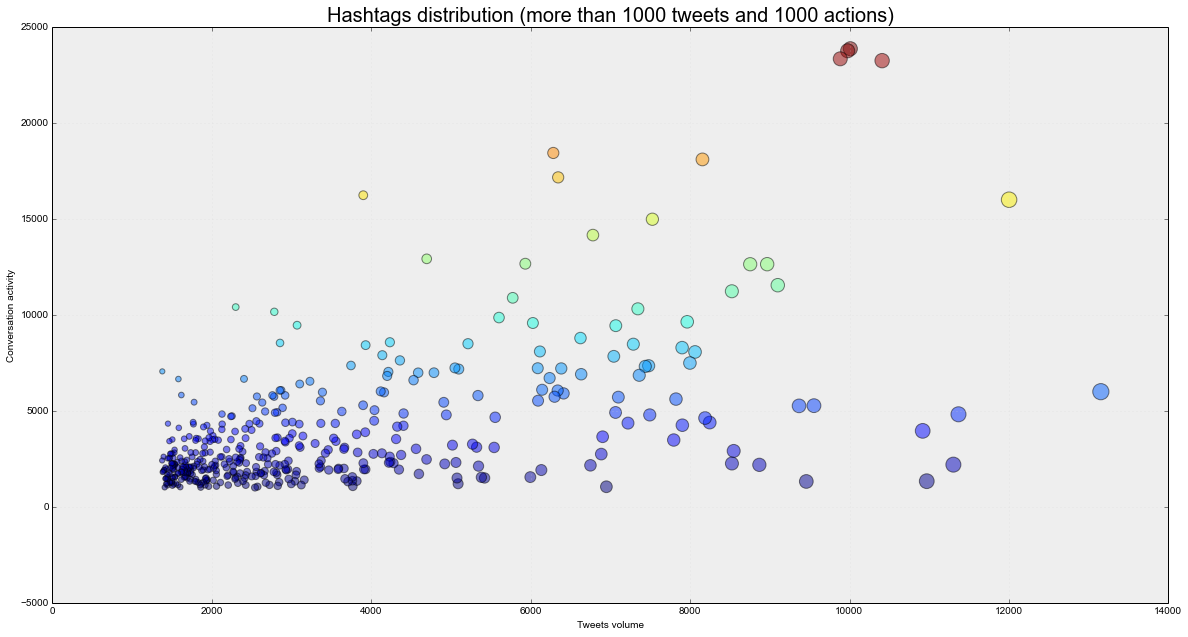
\includegraphics[width=6.0114in,height=3.2114in]{figures/chap3/chapitre3-img8.png}
    \caption{Distribution des 429 hashtags les plus discutés}
\end{figure}


En procédant à l{\textquoteright}étiquetage des hashtags les plus actifs durant l{\textquoteright}année 2012 sur Sina Weibo (figure 2 ci-dessus), nous constatons que la plupart sont associés à des activités commerciales, de loisirs ou de divertissement. Ici nous observons que les usages majoritaires du réseau social Sina Weibo correspondent pour la plupart à ceux d{\textquoteright}autres mass-médias plus traditionnels de par le monde. Le commerce en ligne occupe notamment une place proéminente. La marque de téléphonie mobile chinoise \textit{Xiaomi} est abondamment citée, reflétant son importance croissante dans le marché chinois et surtout sa stratégie commerciale qui cible abondamment les réseaux sociaux avec de nombreux hashtags très discutés (notamment \textit{{\textquotedblleft}Fans de Xiaomi{\textquotedblright} } \#\zh{小米粉丝}\# ). Également, de nombreuses campagnes promotionnelles d{\textquoteright}ouverture ou d{\textquoteright}anniversaire de magasins ont réussi à se hisser dans le jeu de t\^ete des hashtags les plus discutés. Radio-crochets ou chanteurs reconnus, les stars de la télévision et de la chanson sont aussi présents dans le peloton de t\^etes des discussions sur Sina Weibo. Le célèbre chanteur Han Geng notamment compte près d{\textquoteright}une dizaine de hashtags le concernant parmi les 500 les plus discutés (\textit{{\textquotedblleft}Han Geng fait une pub pour Nokia{\textquotedblright}, {\textquotedblleft}Han Geng va en Italie{\textquotedblright}, {\textquotedblleft}Han Geng fait une pub Pepsi{\textquotedblright}, {\textquotedblleft}Han Geng refuse une interview{\textquotedblright}, etc.)} Ici encore, le réseau social agit comme le prolongement des mass média traditionnels, élément-clé des nouvelles stratégies de publicités en ligne, parfois particulièrement agressives comme dans le cas de Han Geng. Les contenus de la télévision sont largement relayés et discutés, notamment les séries télévisuelles. Le cinéma est aussi représenté. Le film comique chinois \textit{Lost in Thailand }sorti en Décembre 2012 dépeint les aventures d{\textquoteright}un chinois en vacances en Thailande. Premier grand succès commercial du box-office chinois, sa popularité se reflète dans l{\textquoteright}importance au sein des discussions en ligne. Les tendances des ventes du livre sont reflétées par de nombreux best-seller sur {\textquotedblleft}l{\textquoteright}amélioration de soi{\textquotedblright} ou la {\textquotedblleft}réussite économique{\textquotedblright}\textit{. }Ce type de hashtags ne se limite pas au support web mais s{\textquoteright}origine directement dans d{\textquoteright}autres médias plus traditionnels. Le gouvernement lui-m\^eme utilise Sina Weibo pour faire passer ses messages avec un hashtag \textit{{\textquotedblleft}information officielle{\textquotedblright} }utilisé notamment pour des démentis publics ou droit de réponse par l{\textquoteright}entreprise Sina, propriétaire du service. également outil de conversation, les discussions sur les réseaux sociaux parlent de la vie de tous les jours. La situation routière et les bouchons dans chaque ville sont un des grands sujets de discussions. Ce sont dans ces échanges quotidiens que se cristallisent plus particulièrement les enjeux politiques et médiatiques des réseaux sociaux. Nouveau café du commerce, les commentaires sur les faits divers et l{\textquoteright}actualité mettent souvent à jour les dysfonctionnements de systèmes politiques, urbains ou légaux. 

Il est intéressant néanmoins de noter que parmi les hashtags les plus discutés, les phénomènes de suppression de contenus par les administrateurs (censure) restent très marginal. Le \textit{China Digital Times} de UC Berkeley maintient une liste des mots interdits sur Sina Weibo depuis plusieurs anneés \citep{Ng2013}. En comparant cette liste de mots censurés à celle des hashtags, nous avons pu voir qu{\textquoteright}aucun des 3000 hashtags les plus utilisés en 2012 n{\textquoteright}a été soumis a une interdiction m\^eme temporaire sur Sina Weibo. Les hashtags les plus sujets à la censure ne sont pas en lien avec des domaines politiques ou des sujets sensibles, mais plut\^ot avec des contenus à caractère pornographique (la pornographie est interdite en Chine). Reflétant les usages majoritaires (commerce, loisirs, etc.), les hashtags véhiculent des contenus souvent moins controversés et les {\textquotedblleft}mots censurés{\textquotedblright} sont plus à m\^eme d{\textquoteright}appara\^itre dans des discussions informelles.



\bigskip


Les limites de chacun des différentes approches nous amènent donc à interroger la pertinence du hashtag comme représentant des mèmes Internet. En effet, la plupart des hashtags semblent être le reflet de campagnes de communication dont la diffusion très planifiée ne laissent que peu de place à des interactions plus spontanées. L'aspect stratégique du hashtag en fait un artefact de campagnes de diffusion, définition seulement partielle et insatisfaisante du mème Internet.  Ainsi, nous préférons écarter l'usage de ce marqueur pour observer les mèmes.

La prochaine section montrera comment une approche par mots-clés, aidée d'outils de contrôle et de vérification pour la qualité des requêtes, peut également donner des résultats satisfaisants.